\documentclass[polish,envcountsect,10pt]{beamer}
    \usepackage[T1]{fontenc}
    \usepackage{polski}
    \usepackage{babel}
    \usepackage{tikz}
    \usepackage{graphicx}
    \usetheme{Warsaw}
    \title{Problem chińskiego listonosza (PCL)}
    \author{184657 Wojciech Panfil}
    \date{Gdańsk, \texorpdfstring{$9.11.2023$}{9.11.2023}}
\begin{document}

\begin{frame}{Test}
    \begin{center}
        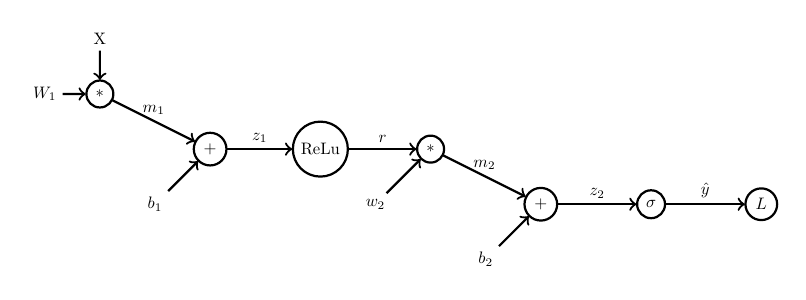
\begin{tikzpicture}[thick,scale=0.7, every node/.style={scale=0.6}]
            \node (X) at (-6,2) {X};
            \node (W1) at (-7,1) {$W_1$};
            \node[draw, circle] (MulA) at (-6,1) {$*$};
            \path [->, above] (X) edge node {} (MulA);
            \path [->, above] (W1) edge node {} (MulA);

            \node (B1) at (-5,-1) {$b_1$};
            \node[draw, circle] (SumA) at (-4,0) {$+$};
            \path [->, above] (MulA) edge node {$m_1$} (SumA);
            \path [->, above] (B1) edge node {} (SumA);
            
            \node[draw, circle] (Relu) at (-2,0) {ReLu};
            \path [->, above] (SumA) edge node {$z_1$} (Relu);

            \node (W2) at (-1,-1) {$w_2$};
            \node[draw, circle] (MulB) at (0,0) {$*$};
            \path [->, above] (Relu) edge node {$r$} (MulB);
            \path [->, above] (W2) edge node {} (MulB);

            \node (B2) at (1,-2) {$b_2$};
            \node[draw, circle] (SumB) at (2,-1) {$+$};
            \path [->, above] (MulB) edge node {$m_2$} (SumB);
            \path [->, above] (B2) edge node {} (SumB);

            \node[draw, circle] (sigma) at (4,-1) {$\sigma$};
            \path [->, above] (SumB) edge node {$z_2$} (sigma);
            
            \node[draw, circle] (ele) at (6,-1) {$L$};
            \path [->, above] (sigma) edge node {$\hat{y}$} (ele);

        \end{tikzpicture}
    \end{center}
\end{frame}

\end{document}